%----------------------------------------------------------------------------------------
%	SLIDE 4.
%----------------------------------------------------------------------------------------
\begin{frame}
\frametitle{Usage in the CMB analysis}

\begin{itemize}
	\item<1-> Main functions for angular power spectrum procession:
	\begin{itemize}
		\item<1-> \texttt{cmb\_spectrum()} : Calculates the power spectrum of an input HEALPix array using \texttt{anafast}.
		\begin{figure}
			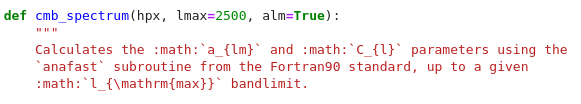
\includegraphics[width=0.7\textwidth]{./images/cmb_spectrum.png}
		\end{figure}
		\item<1-> \texttt{plot\_spectrum()} : Plots the output of \texttt{cmb\_spectrum()}. 
		\begin{figure}
			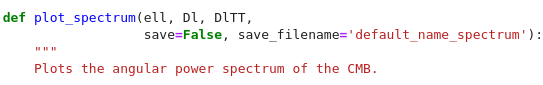
\includegraphics[width=0.7\textwidth]{./images/plot_spectrum.png}
		\end{figure}
	\end{itemize}
\end{itemize}

\end{frame}